\section{A Use Case on Wnt Signaling}


\subsection{Motivation and Problem Statement}

In this use case, we are focusing on a simplified model of the
$\beta$-catenin destruction complex from canonical Wnt signaling. This
complex is highly conserved in animals, and operates from humans to
nematodes to insects to amphibians, regulating the establishment of
the dorso-ventral axis. It is also heavily involved in colon cancer.

A source of complexity in our model is the fact that none of these
enzymes bind directly their substrate. Instead they are loaded onto a
scaffold. Moreover, the scaffold can head-to-tail homopolymerize, in
addition to having three independent binding sites on a second
scaffold, itself capable of dimerization. This allows a highly
degenerate complex of scaffolds, where connection paths or
stochiometries are dynamic. It is this complex that acts as a
super-scaffold to bring the substrate in contact with the
enzymes. Considering both scaffolds contain large regions of disorder
(i.e. chunks of unfolded peptide with high flexibility), it is
sensible to believe an enzyme loaded on one scaffold could modify the
substrate loaded on the neighboring scaffold. Lacking experimental
evidence to suggest a ballpark limit for this reachable horizon, we
leave it constrained: an enzyme will be able to modify any substrate
loaded onto its complex.

%TODO: remove future tense
Having kinases (i.e. enzymes that add a phosphate group) and
phosphatases (i.e. enzymes that remove a phosphate group) loaded on
the same complex will result in unimolecular do-undo loops. Unlike
the classic Goldbeter–-Koshland loop, the sensitivity of this kind of
system will not be simply on the abundance of forward/reverse enzymes,
but now we must consider how they are recruited to complexes, the size
of the complex they get loaded on, and the precedence relations
between the modifications.


\subsection{Experimental Protocol and Queries}

To explore this system, we create a Kappa model with three
parametrizations. The model contains the scaffold proteins Axin1 (Axn)
and APC, the kinases CK1$\alpha$ (CK1) and GSK3$\beta$ (GSK), the
protein phosphatases PP1 and PP2, and the substrate of all these
reactions, $\beta$-catenin (Cat). The destruction complex recruits
Cat through Axn. It then gets phosphorylated at the Serine on position
45 (S45) by CK1. While S45-phosphorylated, it can be phosphorylated at
the Threonine on position 41 (T41) by GSK. While T41-phosphorylated,
it can be phosphorylated on both Serines on positions 37 and 33 (S37 and
S33). Once S37 and S33-phosphorylated, Cat is degraded. Meanwhile, PP1
undoes the phosphorylations of CK1, while PP2 undoes those of GSK.

The three parametrizations are meant to explore the relationship
between phosphatase/kinase ratio and the distribution of do/undo
events per agent. The three parameter pairs are 50/10, 10/10, and
10/50, all in units of number of agents, for the number of kinases and
phosphatases in the model (e.g. 10/50 presents 10 copies of PP1, 10
copies of PP2, 50 copies of CK1, and 50 copies of GSK). The scaffolds
remain at an abundance of 100 each. The models begin with an initial
amount of Cat of 500 agents, and the models are simulated for 500
simulated seconds. We use a universal stochastic bi-molecular binding
rate of $10^{-4}$ per second per agent, a uni-molecular binding rate
of $10^{-2}$ per second, an unbinding rate of $10^{-2}$ per second,
and a catalytic rate of $1.0$ per second. 

For all three parametrizations, we simulate our model and run the
following queries on the resulting traces.

%%%%%%%%%%%%%%%%%%%%%%%%%%%%%%%%%%%%%%%%%%%%%%%%%%%%%%%%%%%%%%%%%%%%%%%%%%%%%%%%

\subsubsection*{Undoing S45, T41, S37 and S33 phosphorylation}
Considering phosphatases undoing the phosphorylation of
sites, does this happen to all agents? Does it happen to just a few agents? What is the distribution of dephosphorylation events per agent? (Figure~\ref{F1})

%match e:{c:Cat(S45{ph/un})}
%return (agent_id{c}, time[e])

%match e:{c:Cat(T41{ph/un})}
%return (agent_id{c}, time[e])

%match e:{c:Cat(S37{ph/un})}
%return (agent_id{c}, time[e])

%match e:{c:Cat(S33{ph/un})}
%return (agent_id{c}, time[e])

\newcommand{\UndoQ}[1]{
\Query{
    \m{match} & e:\Set{ 
      \iAG{c}{\BetaCat}{{#1}^{\,1}_{\Trans{p}{u}}}
    } \\
    \m{return} & \AgentId{c},\, \Time{e}
  }
}

\begin{small}
  \begin{equation*}
    \arraycolsep=7pt
    \begin{array}{cc}
      \UndoQ{S45} & \UndoQ{T41} \\ \\
      \UndoQ{S37} & \UndoQ{S33} \\
    \end{array}
  \end{equation*}
\end{small}

%%%%%%%%%%%%%%%%%%%%%%%%%%%%%%%%%%%%%%%%%%%%%%%%%%%%%%%%%%%%%%%%%%%%%%%%%%%%%%%%

\subsubsection*{Wait times}

What is the distribution of times spent
between the first phosphorylation on an agent, and the time it gets
degraded? (Figure~\ref{F2})

%match i:{+c:Cat}
%and first p:{c:Cat(S45{un/ph})} after i
%and first d:{-c:Cat} after p
%return (agent_id{c}, time[p], time[d])

\begin{small}
\begin{equation}
  \Query{
    \m{match} & i:\Set{  c:\BetaCat+ } \\
    \m{and} & \FirstAfter{p:\Set{
        \iAG{c}{\BetaCat}{{S45}_{\Trans{u}{p}}}
    }}{i} \\
    \m{and} & \FirstAfter{ d:\Set{
        c:\BetaCat-
    } }{p} \\
    \m{return} & \Time{d} - \Time{p}
  } 
\end{equation}
\end{small}

\noindent \textit{About this query.} Agent creation and destruction is
expressed by suffixing agent names with $+$ and $-$,
respectively.

%%%%%%%%%%%%%%%%%%%%%%%%%%%%%%%%%%%%%%%%%%%%%%%%%%%%%%%%%%%%%%%%%%%%%%%%%%%%%%%%

\subsubsection*{Component size and enzyme identity} 
Where do the phosphorylation steps that actually lead to degradation
occur? Do they happen mostly on large complexes? What is
the composition in units of Axn and APC of the complexes where the
phosphorylation events leading to degradation took place? What is the distribution of kinase identifiers for the last phosphorylation events that lead to degradation? (Figure~\ref{F6})

\newcommand{\BigHectorStoryLine}[4]{
\LastBefore{#1:\Set{ 
          \iAG{c}{\BetaCat}{ {#2}^{\,1}_{\Trans{u}{p}}}, \ 
          \iAG{#3}{#4}{c^{\,1}}
    }}{d}
}
\newcommand{\BigHectorStoryRet}[2]{
\AgentId{#2}, \ \Count{ \Component{\StateBefore{#1}}{#2}, \, 
      \STR{Axn}, \, \STR{APC} }
}

%match d:{-c:Cat}
%and last p1:{ c:Cat(S45{un/ph}[1]), k1:CK1(c[1])} before d
%and last p2:{ c:Cat(T41{un/ph}[1]), k2:GSK(c[1])} before d
%and last p3:{ c:Cat(S37{un/ph}[1]), k3:GSK(c[1])} before d
%and last p4:{ c:Cat(S33{un/ph}[1]), k4:GSK(c[1])} before d
%return (
%	agent_id{k1}, count{'Axn', 'APC'}{component[.p1]{k1}},
%	agent_id{k2}, count{'Axn', 'APC'}{component[.p2]{k2}},
%	agent_id{k3}, count{'Axn', 'APC'}{component[.p3]{k3}},
%	agent_id{k4}, count{'Axn', 'APC'}{component[.p4]{k4}}

\begin{small}
\begin{equation}
  \Query{
    \m{match} & d:\Set{ c:\BetaCat - } \\
    \m{and} & \BigHectorStoryLine{p_1}{S45}{k_1}{\CKOne} \\
    \m{and} & \BigHectorStoryLine{p_2}{T41}{k_2}{\GSK}   \\
    \m{and} & \BigHectorStoryLine{p_3}{S37}{k_3}{\GSK}   \\
    \m{and} & \BigHectorStoryLine{p_4}{S33}{k_4}{\GSK}   \\
    \m{return} 
    & \BigHectorStoryRet{p_1}{k_1} \,,\  \\
    & \BigHectorStoryRet{p_2}{k_2} \,,\ \\
    & \BigHectorStoryRet{p_3}{k_3} \,,\  \\
    & \BigHectorStoryRet{p_4}{k_4} \\
  }
\end{equation}
\end{small}

\noindent \textit{About this query.} The \textsf{component} state
measure computes the connected component that contains an agent in a
mixture. It returns a set of agents $S$. The \textsf{count} function
takes such a set $S$ along with $n$ strings denoting agent types and
returns an $n$-tuple of integers indicating how many agents of each
type appear in $S$.


\subsection{Results and Interpretation}

\subsubsection*{Concentration Time Traces}
From the simulator’s output, we get the evolution of the abundance of
Cat through time. In Figure~\ref{F0}, we can see the systems with low phosphatase
behave similarly, even though one has five times the amount of kinases
than the other (blue vs red traces). In contrast, the system with high
phosphatase shows markedly less degradation of Cat; where the other
two system degraded around 450 units, this one has only degraded
23. From this whole-system view, it would seem the amount of
phosphatase is more critical than the amount of kinase: based on the
1:1 system, increasing the kinase five fold has little effect, whereas
increasing the phosphatase has a more dramatic effect.



\begin{figure}[p]
  \centering
  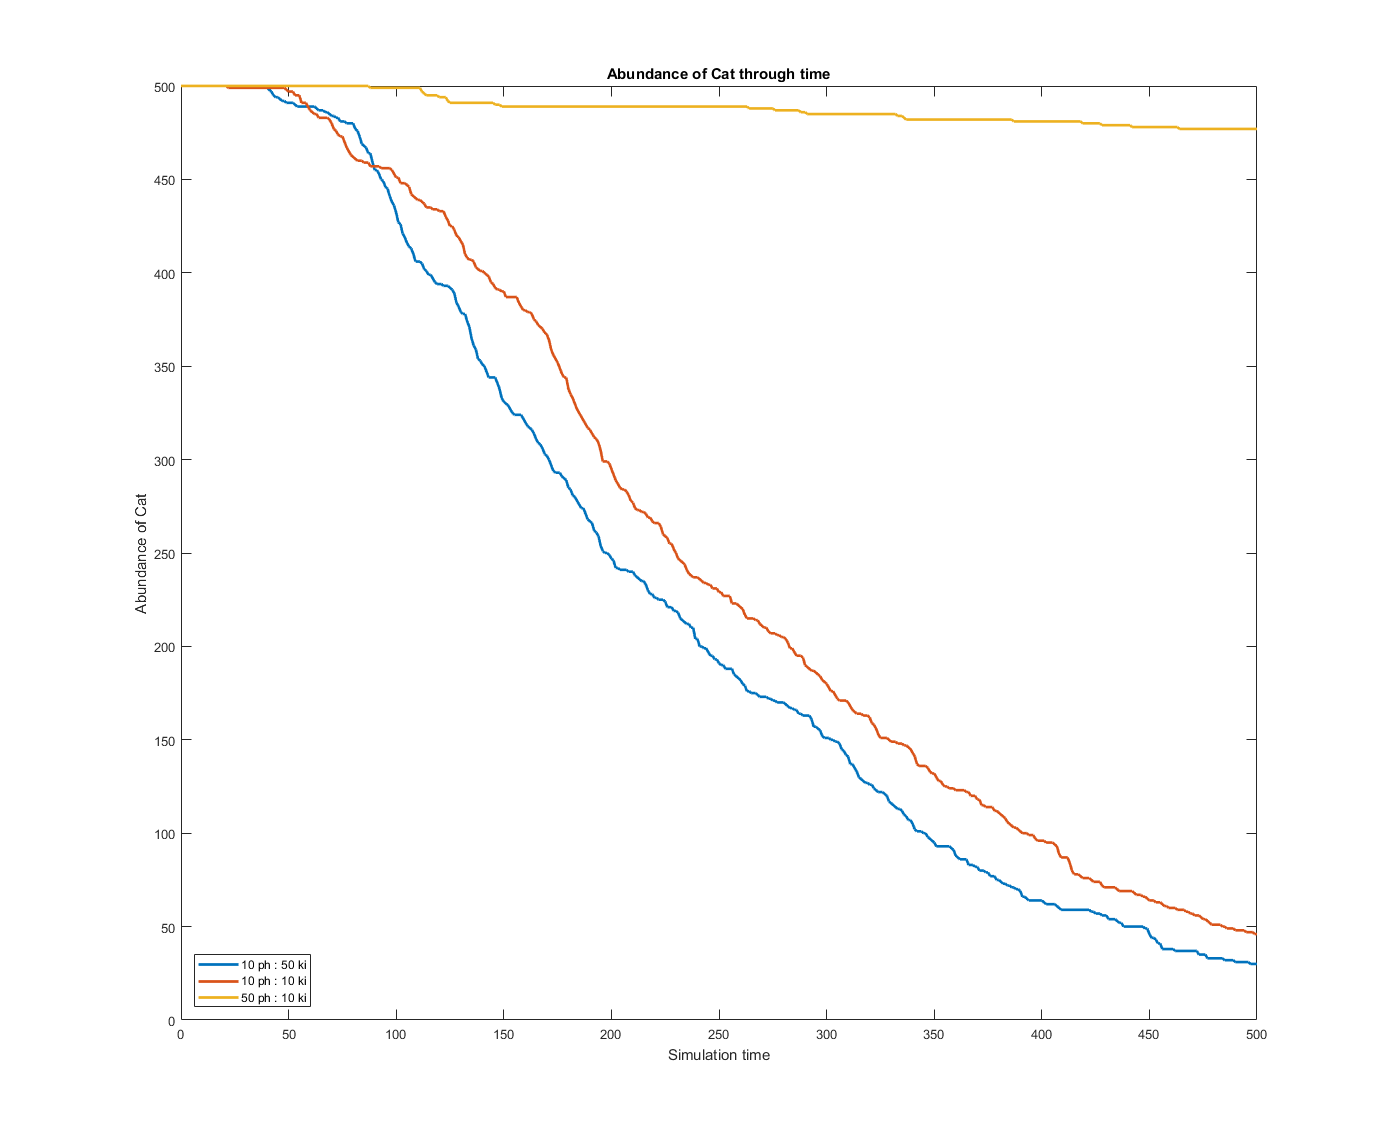
\includegraphics[scale=0.3]{wnt/F0_abundance_of_cat_through_time}
  \caption{Tracking the abundance of agent Cat through the
    simulation. At time $T=0$, the agents are introduced, all in
    monomeric form. The simulation was stopped after five hundred
    simulated seconds. In this legend and throughout the figures, ph
    stands for phosphatase, ki stands for kinase, and the agent
    numbers are presented. Thus ``$10$ ph : $50$ ki'' means the system
    with $10$ units of phosphatase and $50$ of kinase.}
  \label{F0}
\end{figure}

\subsubsection*{Distribution of undo events per agent}

To further study the effect of adding phosphatase, we now look at the
distribution of dephosphorylation events per agent, for each of the
four residues, in Figure~\ref{F1}. S45 is the first residue to
phosphorylate in the causal chain leading to degradation. Based on the
1:1 system, is is surprising to see increasing the phosphatase level
five fold maintains a similar total number of dephosphorylation events
(compare curves’ integrals). However, their distribution is quite
different; under 1:1 conditions the dephosphorylation events happen
mostly on a sub-population of agents, while under 5:1 conditions they
are happening more widespread. Interestingly, the increasing the
amount of kinase to 1:5 led to decrease in dephosphorylation
events. It is also worth noting, the 1:1 saw almost 30 thousand
dephosphorylation events of S45, with some specific agents getting
dephosphorylated almost 800 times. This would imply a comparable
number of phosphorylation events for that specific copy of Cat.

To answer the question that motivated this query, under 1:5 regime,
most agents don’t get sabotaged by the phosphatase; the blue line is
quite flat. Decreasing the amount of kinase however changes this, and
under a 1:1 regime some agents get undone several times, a quarter
seeing upwards of hundreds of undo events (e.g. from id 300
onward). Increasing the phosphatase to a 5:1 regime further
exacerbates this, with over half the agents receiving undo events
hundreds of times. The unavailability of phosphorylated S45 in turn
inhibits the phosphorylation of T41, and so forth to S37 and S33. It
is worth noting that, based on the 1:1 system, increasing the
phosphatase five fold decreases the number and extend of advanced
dephosphorylation events, such as S33 and S37. Paradoxically,
increasing the kinase five fold has this same effect. We attribute the
former to decreased availability of the intermediate phosphorylated
states (i.e. if T41 is not phosphorylated, S37 can’t be
phosphorylated, ergo can’t be dephosphorylated), and the latter to
increased throughput to degradation (i.e. Cat is not around for long
enough to get dephosphorylated, as once it gets phosphorylated it
extremely quickly proceeds to get degraded).

We call attention to the number of agents whose final sites got
dephosphorylated (Figure~\ref{F1}), vs the number of agents who got
degraded (Figure~\ref{F0}). The 1:5 or 1:1 systems both degraded over
450 agents each, but the former undid around 160 agents while the
latter undid over 350. For the 1:5 and 5:1 systems, both undid around
160 agents, but the former degraded over 450 agents while the latter
less than 50. This argues the notion of efficiency (e.g. minimizing
the amount of undo steps) can’t readily be inferred from the
throughput of the system.


\begin{figure}[p]
  \centering
  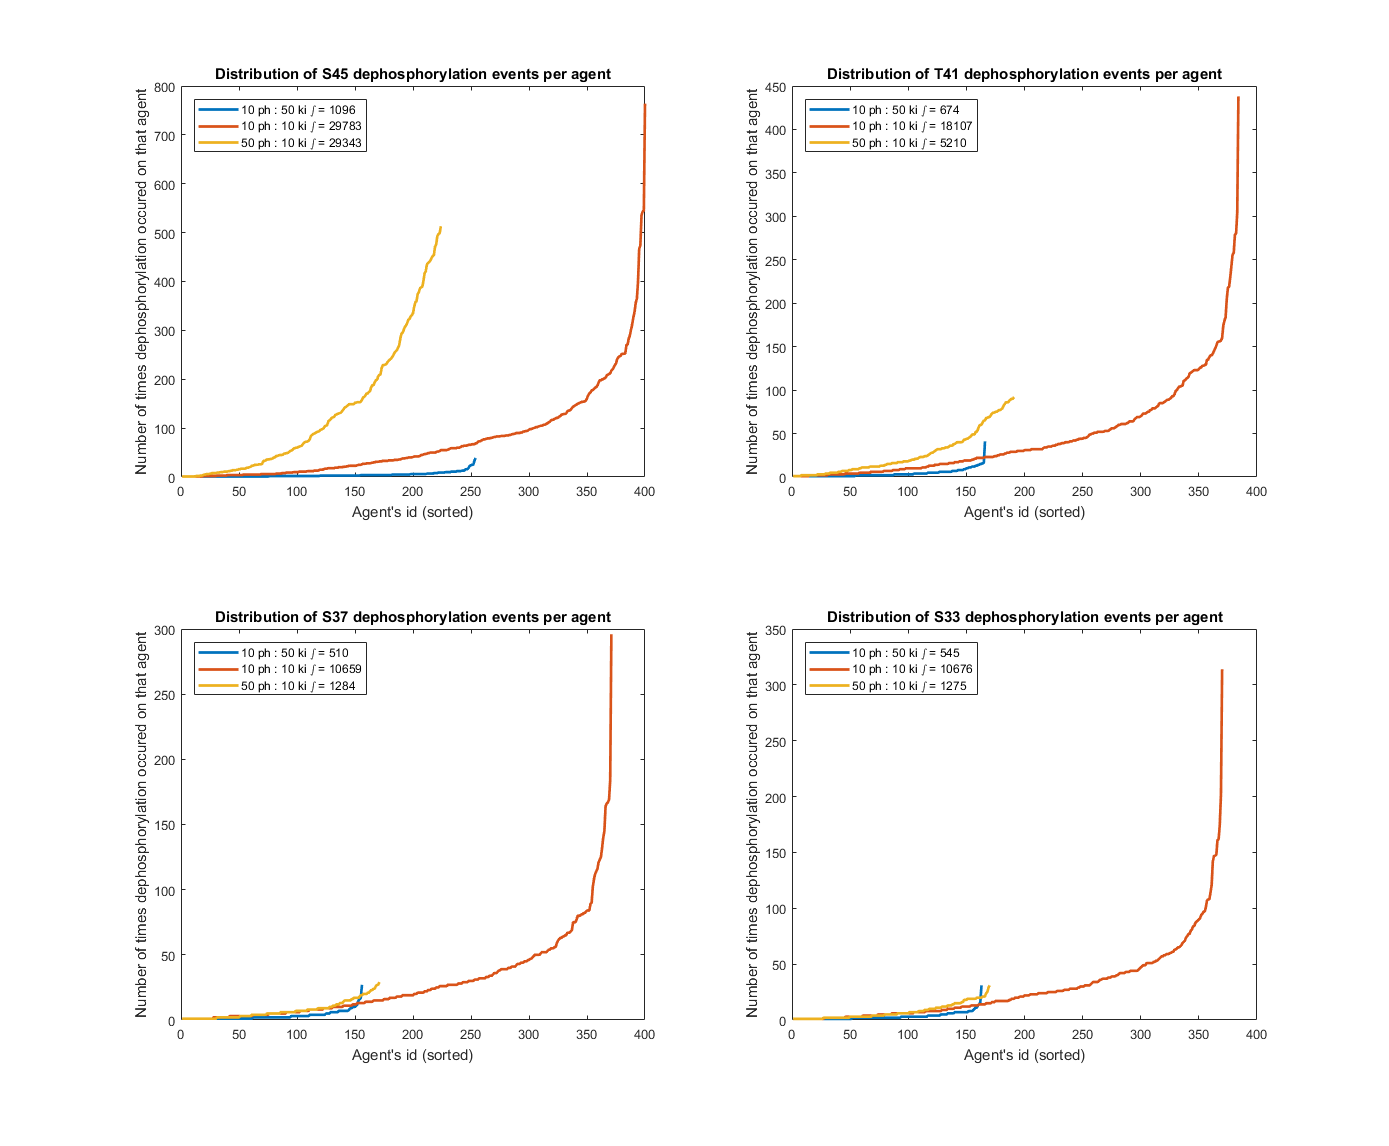
\includegraphics[scale=0.35]{wnt/F1_distribution_dephosphorylations_per_agent}
  \caption{Distribution of dephosphorylation events per agent. Each
    time an agent gets dephosphorylated, its ID is registered. After
    sorting, we plot the distribution of these IDs for all four
    residues in the three parameter regimes. The area under the curve
    is also presented on each legend.}
  \label{F1}
\end{figure}


\subsubsection*{Wait times}
Looking at the distribution of wait times (Figure~\ref{F2}), from first phosphorylation
to degradation, we note the bulk of degradation events occur rapidly,
in less than $50$ seconds. Worth noting that, from the 1:1 regime,
increasing the amount of kinase five fold marginally reduced wait
times. Increasing the amount of phosphatase produced such sparse
results that little can be said.

\begin{figure}[p]
  \centering
  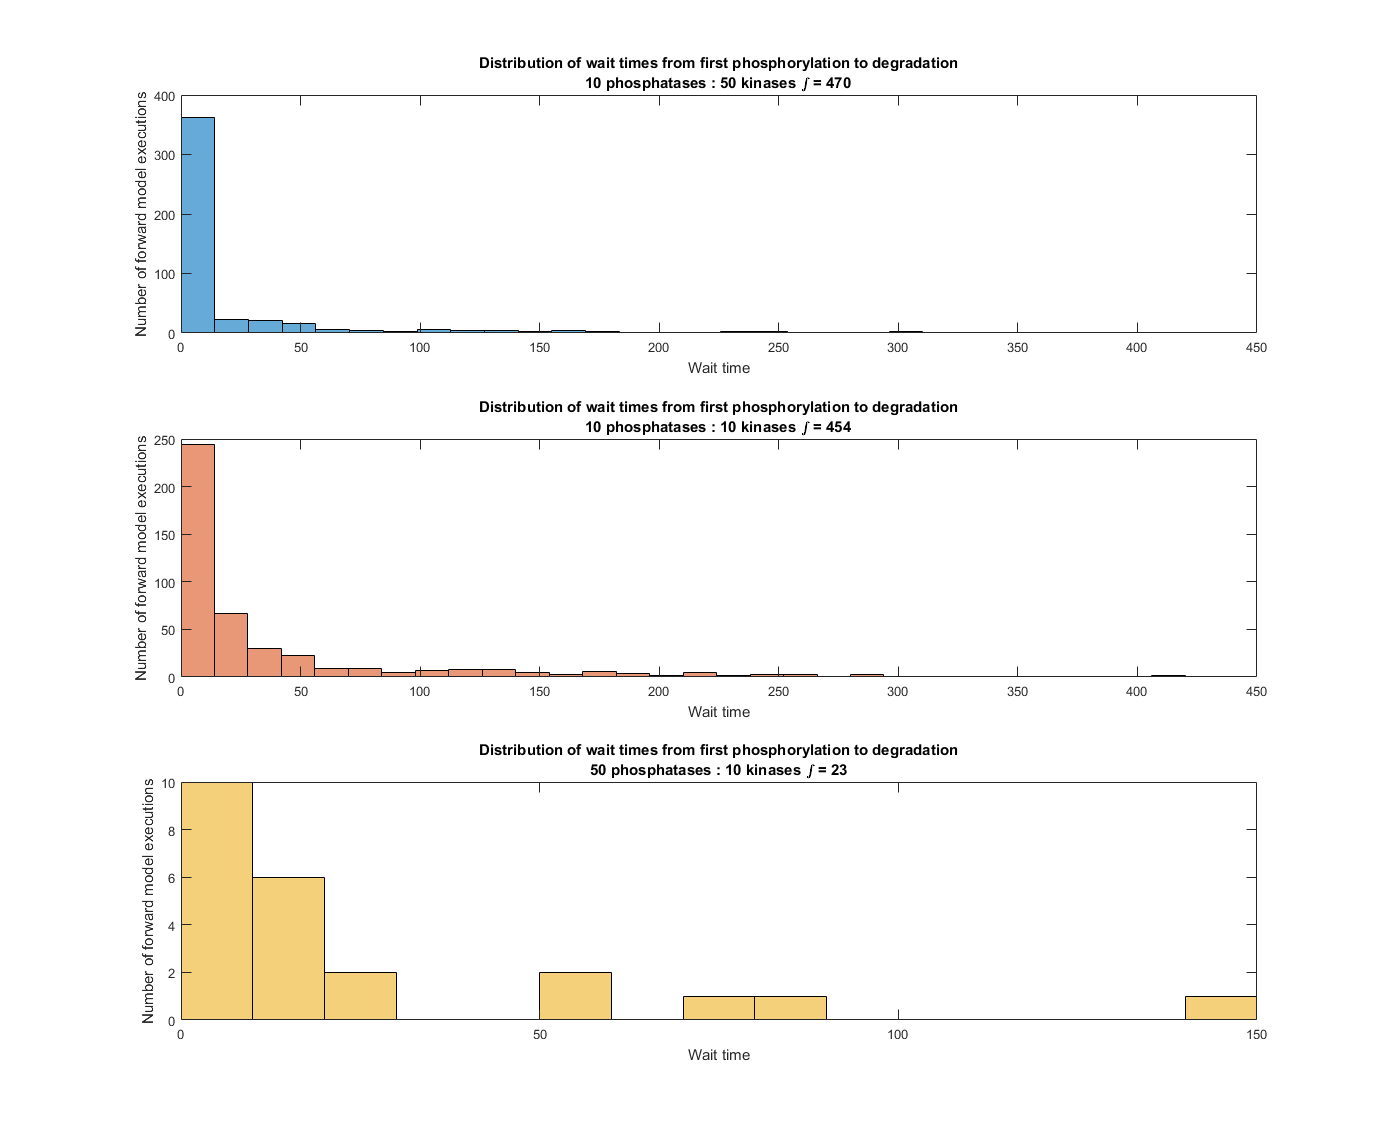
\includegraphics[scale=0.35]{wnt/F2_wait_times}
  \caption{Distribution of wait times from first phosphorylation until
    degradation. The sum of the bins is presented in the title of each
    plot. The number of bins was determined by MatLab's automatic
    algorithm. A “forward model execution” means a degradation event.}
  \label{F2}
\end{figure}

\subsubsection*{Distribution of dephosphorylation times}

We wondered if the dephosphorylation events could be due to transient
recruitment of phosphatases to complexes, if the system operated
mostly in the forwards (phosphorylation) route, with occasional bursts
of dephosphorylation activity. We therefore plotted the distribution
of dephosphorylation events in time (Figure~\ref{F3}).

Based on the system with 1:1, increasing the amount of kinase five
fold to 1:5 flattened the distribution of dephosphorylation times. In
contrast, increasing the amount of phosphatase had the opposite
effect, with the bulk of events happening after half the simulation
had elapsed. For the 1:1 system, we interpret the early stages as
revealing an initialization wait: scaffold complexes are being
assembled, and so the phosphatase events are not happening as
fast. Once these are assembled, the system enter a more stable
regime. However, eventually the abundance of Cat is low enough that
the system becomes less active. These regimes match the different
regions in Figure~\ref{F0}, with a slow decline before time $T=100$, a
steady decline through to $T=400$, then a slow decline onward.


\begin{figure}[p]
  \centering
  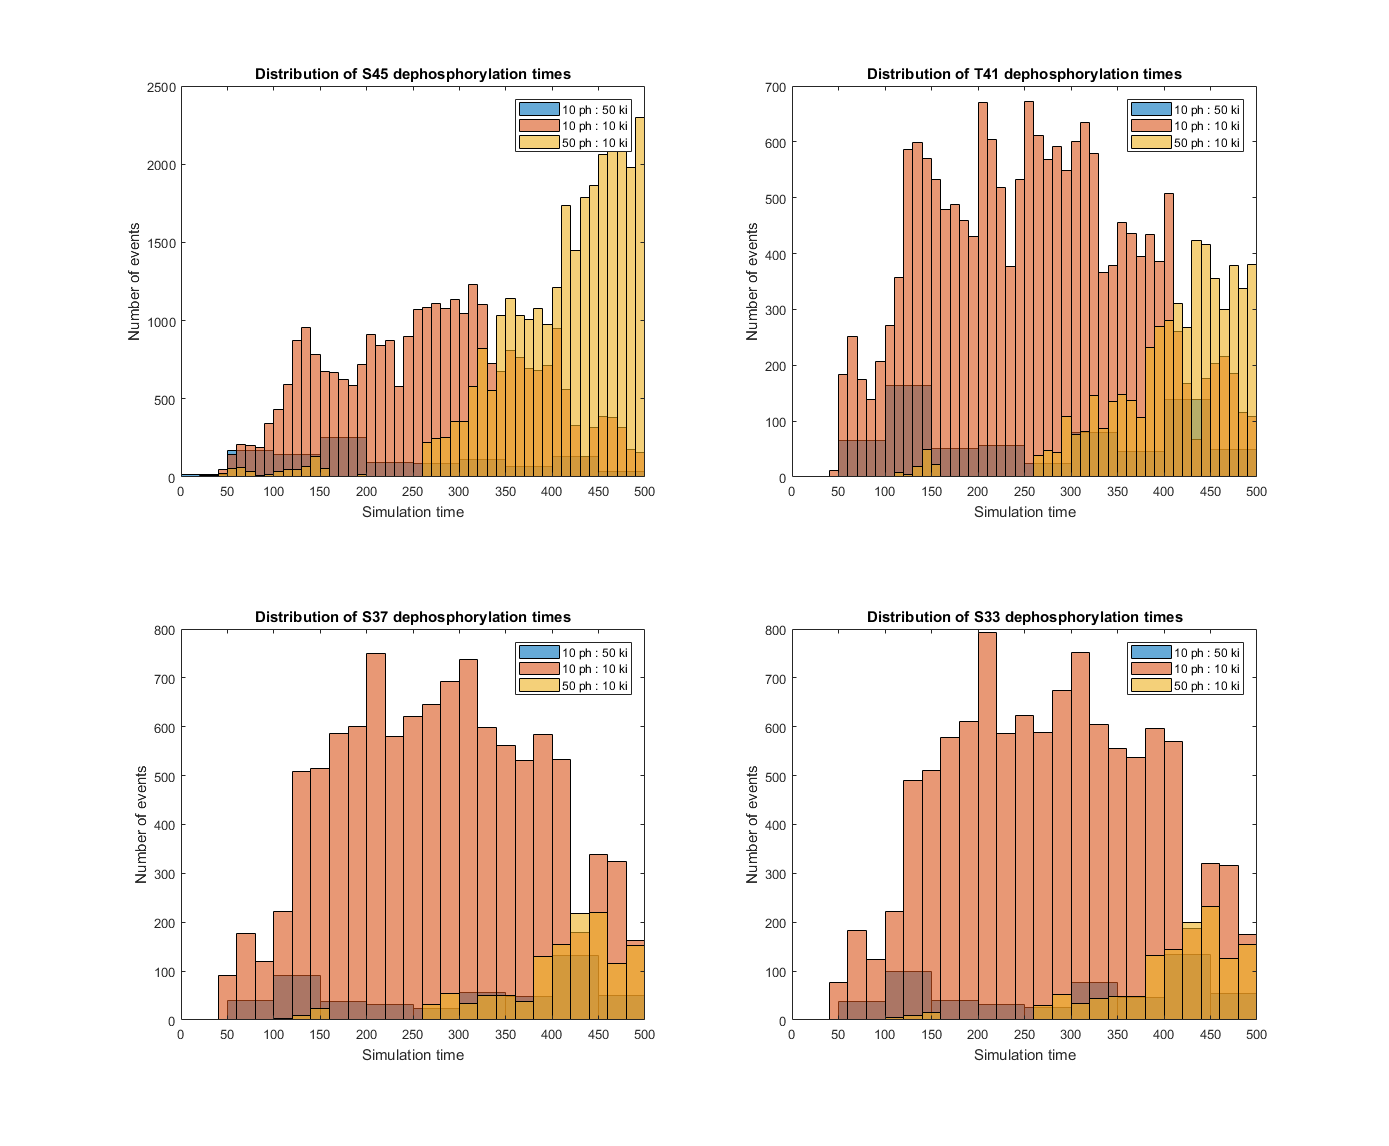
\includegraphics[scale=0.35]{wnt/F3_distribution_of_dephosphorylations_in_time}
  \caption{Distribution of dephosphorylation events in time.}
  \label{F3}
\end{figure}

\subsubsection*{Responsibility of final phosphorylation}

We next turned to the question of how did enzymes contribute to the
forward kinetics, those of phosphorylation. In Figure~\ref{F4}, we
show how many times a particular enzyme produced the final
phosphorylation before degradation. In Figure~\ref{F5}, we show the
same but as a fraction of all degradation events. Under both 1:5 and
1:1 regimes, the distributions are fairly flat. In contrast, under the
5:1 regime, it is only a few enzymes that contributed to the actual
degradation of Cat; all the other thousands of phosphorylation and
dephosphorylation events (Figure~\ref{F1}) were caught in the do-undo
cycle.

\begin{figure}[p]
  \centering
  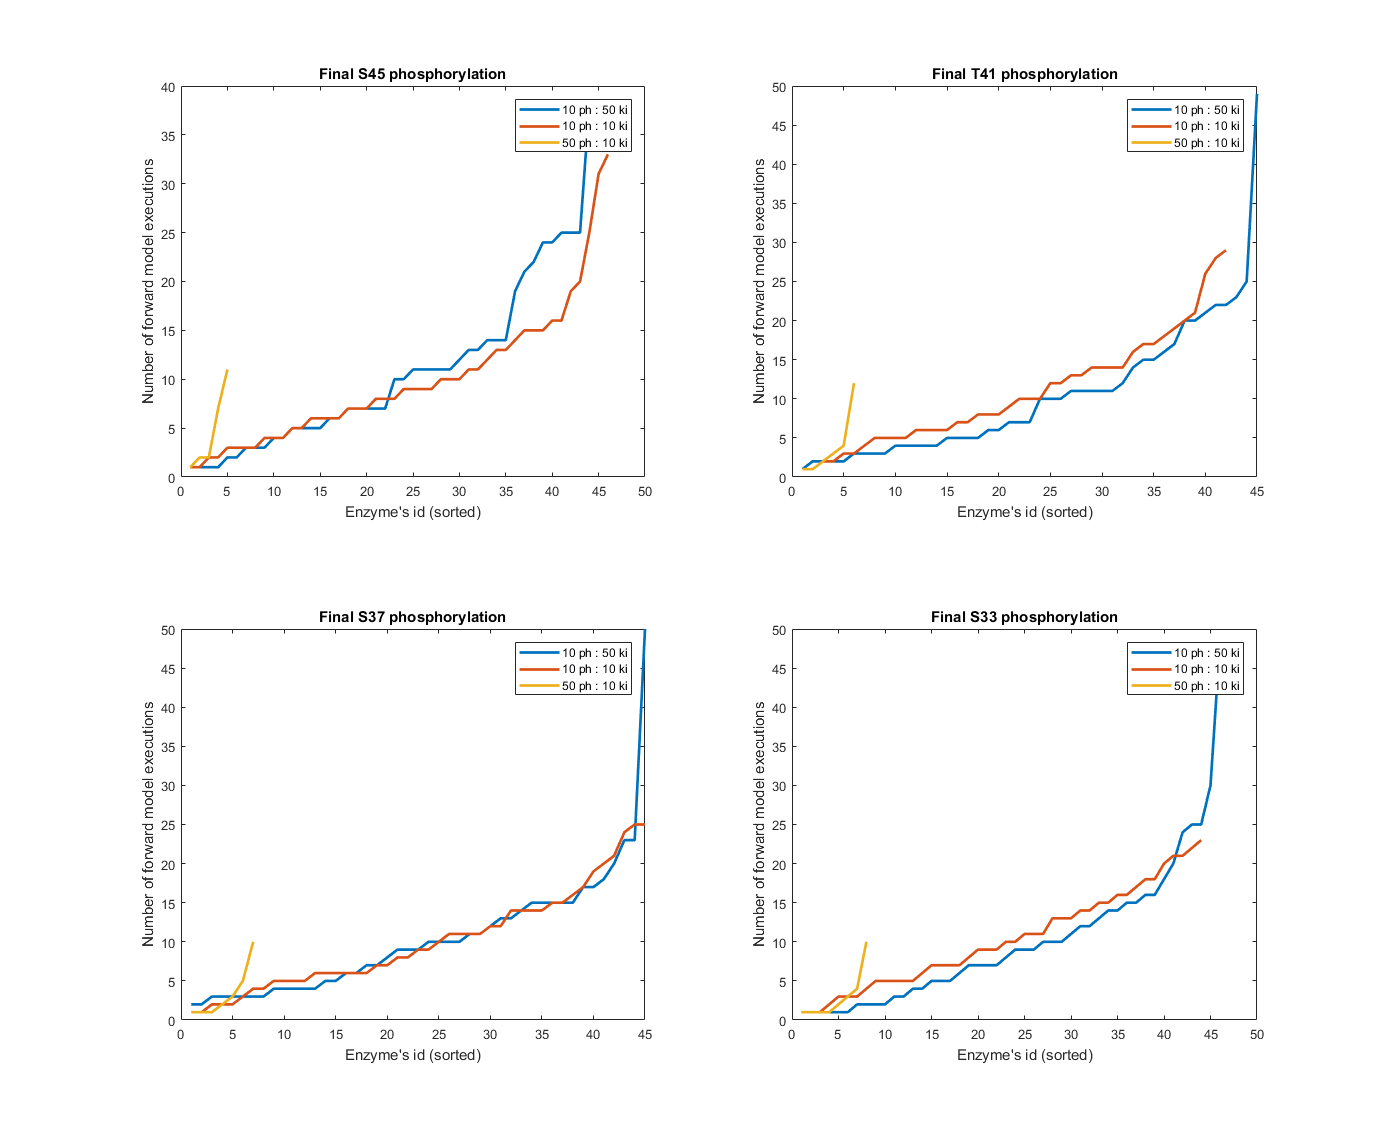
\includegraphics[scale=0.35]{wnt/F4_final_phosphorylation_enzyme_id_absolute}
  \caption{Identifiers of enzymes responsible for the final
    phosphorylation step taken before degradation, for all four
    residues. Presented are absolute counts per enzyme id.}
  \label{F4}
\end{figure}


\begin{figure}[p]
  \centering
  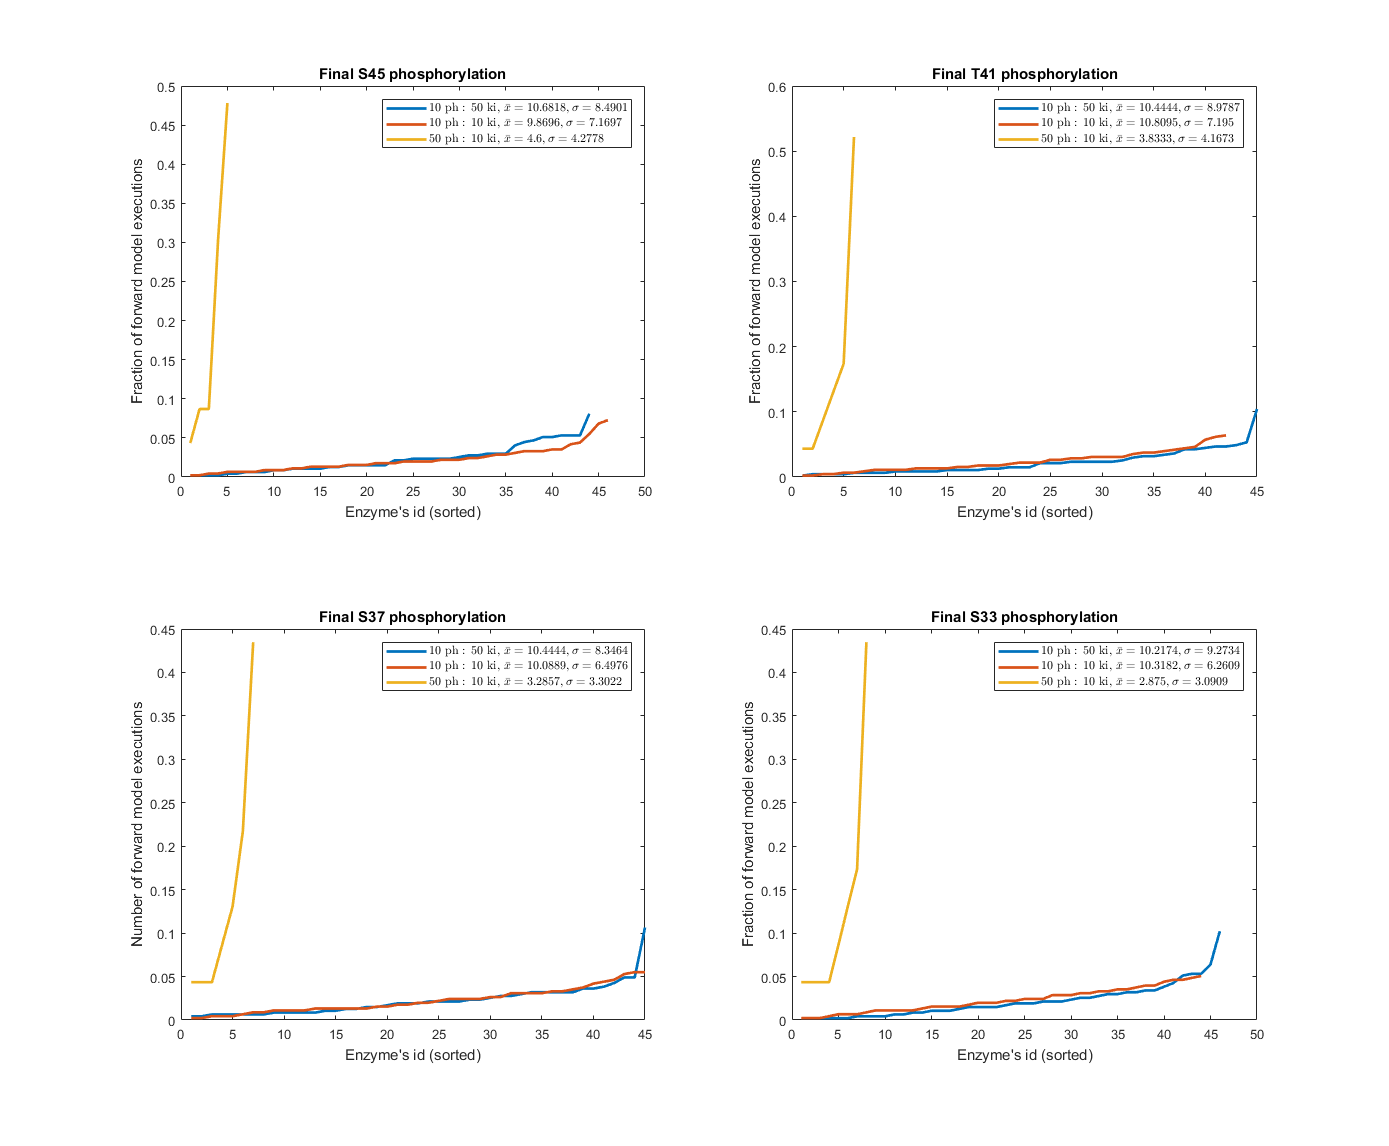
\includegraphics[scale=0.35]{wnt/F5_final_phosphorylation_enzyme_id_fraction}
  \caption{Identifiers of enzymes responsible for the final
    phosphorylation step taken before degradation, for all four
    residues. Presented are fractions of overall contribution per
    enzyme id. $\bar{x}$ represents the average number of final
    substrate modification per enzyme, $\sigma$ the standard
    deviation.}
  \label{F5}
\end{figure}


\subsubsection*{Complex composition: changes in ratio}

Another way of looking at the question of what complex contributes
most to the degradation of Cat is to query the size of the complex at
the last phosphorylation event before degradation. Taking S45 as
representative of all the other residues, we plot the size of the
complex, in terms of Axn and APC. Overall, we see a broad distribution
of sizes, with a some phosphorylation events occurring in large
complexes (i.e. $>80$ Axn, $>40$ APC), but a significant number occurring
in far smaller complexes (i.e. $<10$ Axn, $<10$ APC). Changing the
parameter regime of kinase to phosphatase does not seem to alter this
behavior significantly, though for the 1:5 system the number of events
is low enough that it is difficult contrasting against the behavior of
the other systems. As for the other residues, their behavior is
extremely similar to the one shown for S45.

\begin{figure}[p]
  \centering
  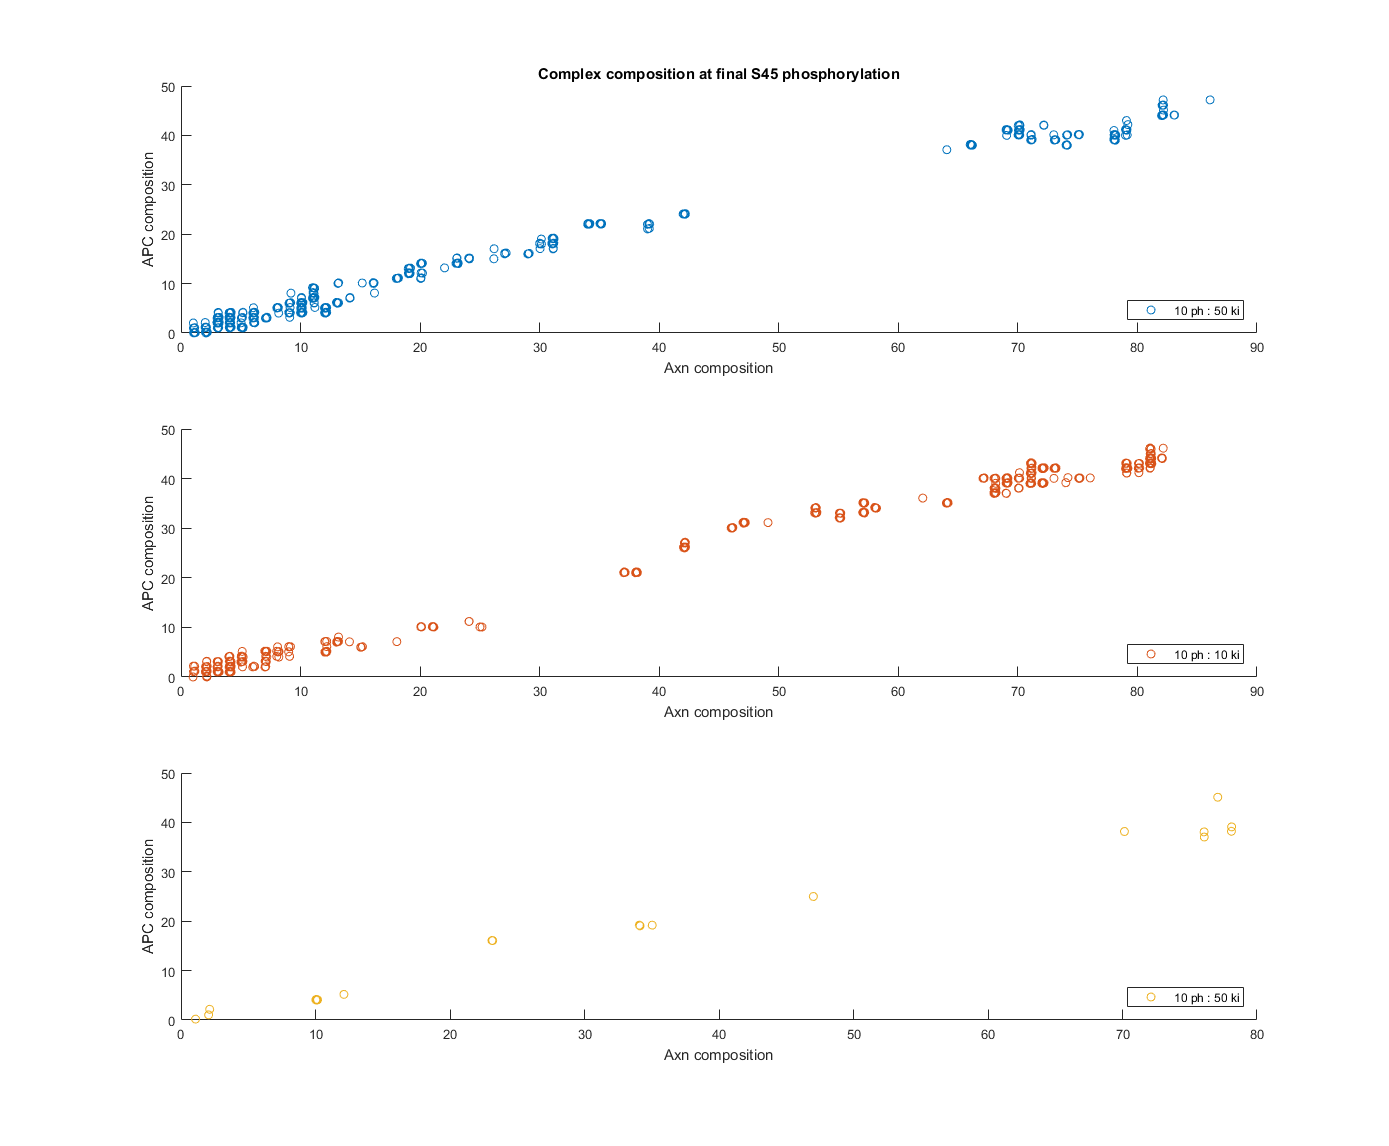
\includegraphics[scale=0.35]{wnt/F6_complex_composition_final_S45}
  \caption{Composition of the complex, in terms of Axn and APC
    components, at the last event where Cat got S45 phosphorylated
    before being degraded. The number of points is the number of
    degradation events, per system. This scatter plot’s points have
    been nudged with a random noise factor of 0.2 to increase visual
    perception of discrete points where the data overlap.}
  \label{F6}
\end{figure}


\subsubsection{Complex composition: all four on the same component?}

For the final query, we wonder if all four final phosphorylation
events occur on the same complex. Given the short wait time
(Figure~\ref{F2}), one might expect so, but the number of
dephosphorylation events is so large (Figure~\ref{F1}), it could be
well that a substrate is partially modified on one complex,
subsequently modified on another, finalized in yet another. Lacking a
metric by which we can compare complexes for distance, we instead
compare complex compositions as a proxy.

Seeing how overwhelmingly, for each specific Cat’s modifications, the
S45 phosphorylation events happened on complexes of the same Axn and
APC composition as the T41 phosphorylation events, as the S37
phosphorylation events, as the S33 phosphorylation events, we feel
confident in claiming all four steps occurred on the same
complex. This agrees well with the observation that the wait times are
fairly short (Figure~\ref{F3}). We did not see an appreciable
difference for the other parameter regimes.

\begin{figure}[p]
  \centering
  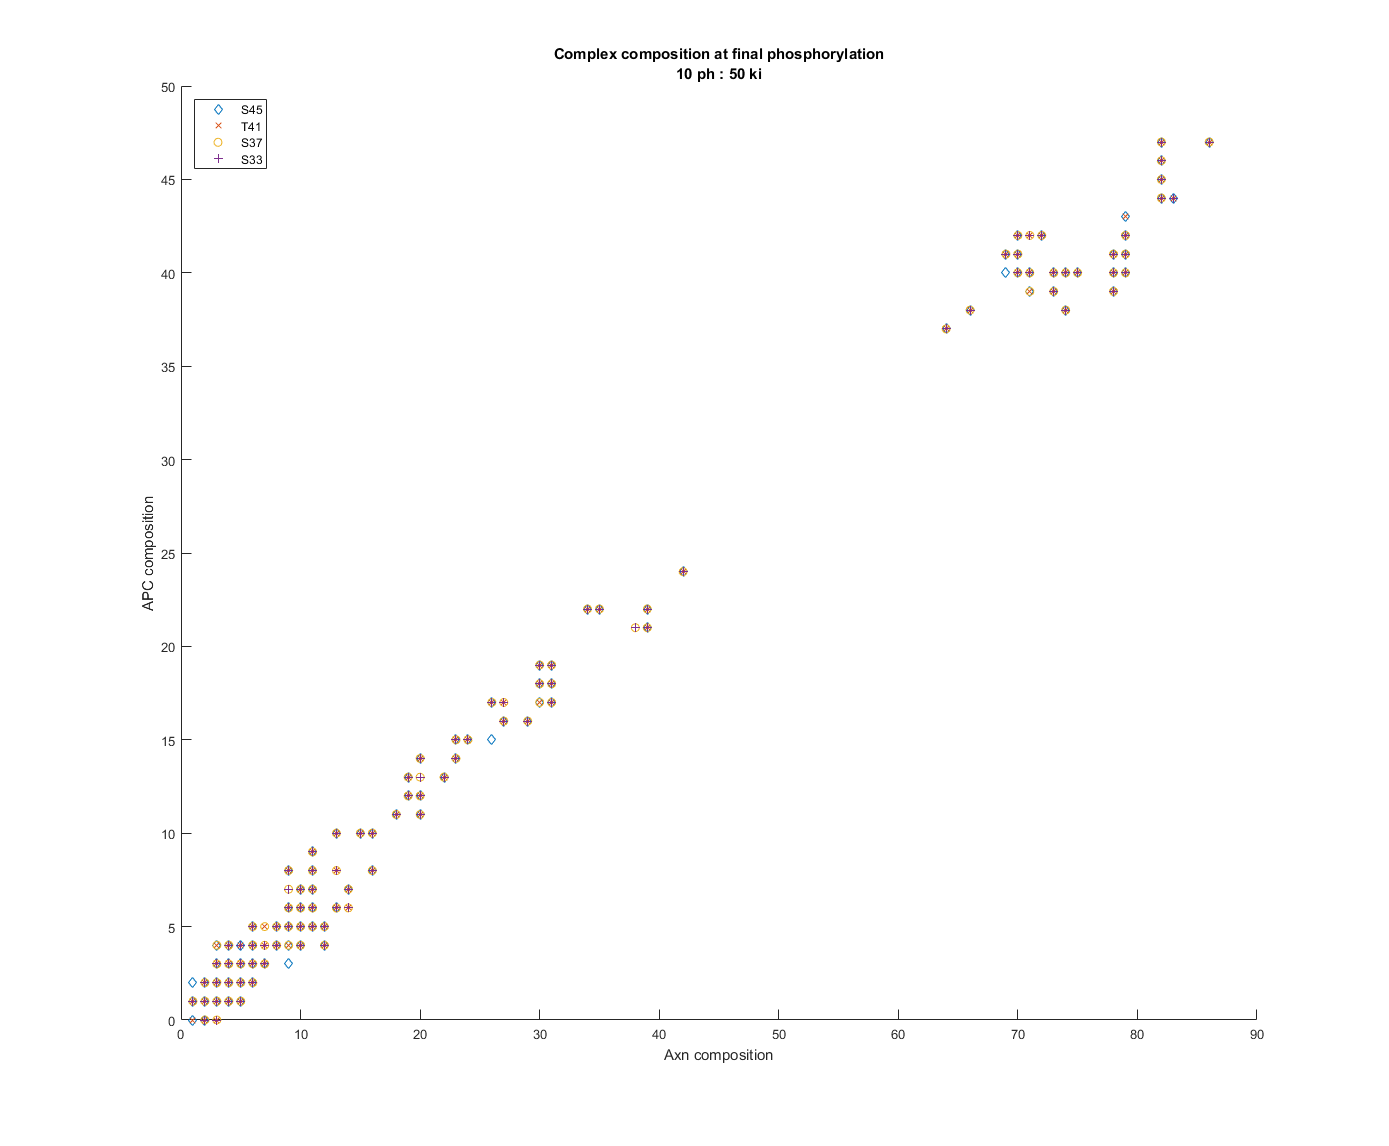
\includegraphics[scale=0.32]{wnt/F10_complex_composition_10_50}
  \caption{Complex composition at the time of the last phosphorylation
    for the 1:5 system. All four residues are shown. A diamond
    superposed with a cross superposed with a circle superposed with a
    plus sign indicates all four modifications for a specific copy of
    Cat occurred on a complex of the same composition in terms of Axn
    and APC. We interpret this as having occurred on the exact same
    complex.}
  \label{F10}
\end{figure}

\subsection{Conclusions}

\begin{enumerate}
\item The number of undo events does not inform us of overall
  throughput (Figure~\ref{F0} and Figure~\ref{F1}).
\item How a step may be affected by changing abundances depends
  greatly on its upstream context (Figure~\ref{F1}).
\item Entities that got degraded waited a short while since their
  first modification (Figure~\ref{F2}), and yet most modifications
  were futile (Figure~\ref{F1}).
\item How the kinetics of dephosphorylation are distributed through
  time changes on the ratio of forward to reverse enzymes
  (Figure~\ref{F3}), with some regimes showing behavior absent in
  others.
\item We can’t argue that a specific enzyme performs the bulk of the
  effective (i.e. final) phosphorylation events (Figures~\ref{F4} and
  \ref{F5}), unless the reverse enzyme is too high, point at which a
  few enzymes contribute the bulk of the events.
\item We can’t argue that giant complexes, nor small complexes, nor
  medium complexes, are the sole entities responsible for performing
  the effective (i.e. final) phosphorylation events
  (Figure~\ref{F6}); %F6-9
  the distribution of complexes is wide, and they all contribute to
  the kinetics.
\item Once an agent starts getting modified, it keeps getting modified
  and finishes getting modified within the same complex
  (Figure~\ref{F10}); % (F10-12)
  a specific agent’s modification is not happening piece-meal over a
  large set of complexes, but rather quickly (Figure~\ref{F2}), on the
  same complex (Figure~\ref{F10}), % (F10-12)
  by a large set of enzymes (Figures~\ref{F4} and \ref{F5}).
\end{enumerate}